\section{Calculations}
\label{sec:calc}
The Rotation matrices for the 24 common Euler and fixed angleset conventions are all defined in appendix B in the course book\cite{bib1}. These can be used directly to calculate the rotation matrices for a given angleset based on three input angles. The equations for calculating the angles based on the rotation matrix are not documented fully in the book however.\\

An example of how to derive these equations are shown below. This example is based on the  angleset Euler XYZ shown in equation \eqref{eq:eq0}. 

\begin{equation}
R_{{X^I}{Y^I}{Z^I}}(\alpha,\beta,\gamma) =
\begin{bmatrix}
\cb \cg & -\cb \sg & \sb \\
\sa \sb \cg + \ca \sg & -\sa \sb \sg + \ca \cg & -\sa \cb \\
-\ca \sb \cg + \sa \sg & \ca \sb \sg + \sa \cg & \ca \cb
\end{bmatrix}
\label{eq:eq0}
\end{equation}


The input angles are found according to equation \eqref{eq:eq1}, \eqref{eq:eq2} and \eqref{eq:eq3} by using the atan2-function.
\begin{align}
\beta  &= Atan2(sin(\beta ),cos(\beta ))   \label{eq:eq1} \\
\alpha &= Atan2(sin(\alpha ),cos(\alpha )) \label{eq:eq2} \\
\gamma &= Atan2(sin(\gamma ),cos(\gamma )) \label{eq:eq3}
\end{align}

The Atan2-function takes two parameters, namely the sine and cosine element of a variable. From equation \eqref{eq:eq1} the sine part of $\beta$ is derived as shown in equation \eqref{eq:eq4} and the cosine part in equation \eqref{eq:eq5}.

\begin{equation}
sin(\beta )=r_{13}
\label{eq:eq4}
\end{equation}
\begin{equation}
cos(\beta )=\sqrt{r{_{11}}^{2} + r{_{12}}^{2}}
\label{eq:eq5}
\end{equation}

This is derived as shown in equation \eqref{eq:eq6} and makes it possible to rewrite equation \eqref{eq:eq1} to equation \eqref{eq:eq7}.

\begin{align}
r{_{11}}^{2} + r{_{12}}^{2} &= cos(\beta )^2cos(\gamma )^2+cos(\beta )^2sin(\gamma )^2 \nonumber \\
 &=cos(\beta )^2(cos(\gamma )^2+sin(\gamma )^2) \nonumber \\
 &=cos(\beta )^2 \label{eq:eq6}
\end{align}

\begin{equation}
\beta = Atan2(r_{13,\sqrt{r{_{11}}^{2} + r{_{12}}^{2}}})
\label{eq:eq7}
\end{equation}


Solving $cos(\beta)$ makes it possible to solve equation \eqref{eq:eq3} and \eqref{eq:eq4} in an equal manner:

\begin{align}
sin(\alpha ) &= \tfrac{-r_{23}}{cos(\beta )} \nonumber \\
cos(\alpha ) &= \tfrac{r_{33}}{cos(\beta )}  \nonumber \\
\alpha &= Atan2(\tfrac{-r_{23}}{cos(\beta )},\tfrac{r_{33}}{cos(\beta )}) \label{eq:eq10}
\end{align}

\begin{align}
sin(\gamma ) &=\tfrac{-r_{12}}{cos(\beta )} \nonumber \\
cos(\gamma ) &= \tfrac{r_{11}}{cos(\beta )} \nonumber \\
\gamma &= Atan2(\tfrac{-r_{12}}{cos(\beta )},\tfrac{r_{11}}{cos(\beta )}) \label{eq:eq13}
\end{align}

As equation \eqref{eq:eq10} and \eqref{eq:eq13} divides by $cos(\beta)$, having $\beta$ at angles equal to $-90^{\circ}$ or $90^{\circ}$ makes it impossible to derive $\alpha$ and $\gamma$ with these equations. In these cases $\alpha$ is chosen to $0^{\circ}$ making it possible to solve all angles as shown in equation \eqref{eq:eq14} and \eqref{eq:eq15}.

\begin{align}
\beta &= -90^{\circ} \nonumber \\
\alpha &= 0          \nonumber \\
\gamma &= Atan2(-r_{32},r_{31}) \label{eq:eq14}
\end{align}

\begin{align}
\beta &= 90^{\circ} \nonumber \\
\alpha &= 0         \nonumber \\
\gamma &= Atan2(r_{32},-r_{31}) \label{eq:eq15}
\end{align}


The above special cases are an example of equations using $cos(\beta)$. All the conventions can be solved in a similar manner, though some of them uses $sin(\beta)$ to solve $\alpha$ and $\gamma$ angles. In these, the special cases are at $\beta$ angles of $0^{\circ}$ or $180^{\circ}$.\\
Moreover, the Euler XYZ angleset convention is equal to the Fixed ZYX angleset convention. This holds true for all Euler and Fixed anglesets, thus reducing the 24 conventions to 12 unique. Our program solves 6 of these as shown in table \ref{tab:anglesets}.

\begin{table}[H]%
\centering
\begin{tabular}{|c|c|}
\hline
Euler ZYX & Fixed XYZ \\
\hline
Euler XYZ & Fixed ZYX \\
\hline
Euler XZY & Fixed YZX \\
\hline
Euler YXZ & Fixed ZXY \\
\hline
Euler ZXZ & Fixed ZXZ \\
\hline
Euler ZYZ & Fixed ZYZ \\
\hline
\end{tabular}
\caption{Implemented angleset conventions}
\label{tab:anglesets}
\end{table}

%\begin{figure}[H]
%  \centering
%  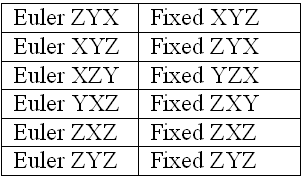
\includegraphics[scale=0.5]{tex/figure_17.png} 
%  \caption{}
%  \label{fig:table1}
%\end{figure}
